\documentclass{article}
\usepackage{authblk}
\usepackage{float,graphicx}
\usepackage[figuresright]{rotating}
\usepackage[usenames,dvipsnames]{color}
\usepackage{makeidx}
\usepackage{dcolumn}% Align table columns on decimal point
\usepackage{bm}% bold math
\usepackage{url}
\usepackage[toc,page,titletoc]{appendix}
\usepackage[small,bf]{caption}
\usepackage{tabulary}
\usepackage{booktabs,multirow,dcolumn,bigdelim}
\newcommand{\otoprule}{\midrule[\heavyrulewidth]}
\usepackage[pdftex,plainpages=false,pdfpagelabels,backref,pdfborder={0 0 0}]{hyperref}
\usepackage{moresize}
\usepackage[scaled]{helvet}
\usepackage[text={6.5in,8.75in},headheight=15pt,centering]{geometry}
\usepackage{fancyhdr}
\pagestyle{fancy}
\usepackage{amsmath}
\usepackage{amssymb}
\usepackage{cite}
\usepackage{amssymb}
\usepackage{textgreek}
\usepackage{cleveref}
%\usepackage{float}
\usepackage{makeidx}
%\usepackage{hyperref}
\usepackage{hyperref}
\usepackage{indentfirst}
\hypersetup{
    colorlinks,
    citecolor=black,
    filecolor=black,
    linkcolor=black,
    urlcolor=black
}
\usepackage{url}

%\documentclass{article}
%\usepackage[utf8]{inputenc}
%\documentclass[sigconf, authordraft]{acmart}
%\usepackage{booktabs} % For formal tables
% Copyright
%\setcopyright{none}
%\setcopyright{acmcopyright}
%\setcopyright{acmlicensed}
%\setcopyright{rightsretained}
%\setcopyright{usgov}
%\setcopyright{usgovmixed}
%\setcopyright{cagov}
%\setcopyright{cagovmixed}
%\usepackage{float,graphicx}
%\usepackage{cite}

\parskip5pt

\begin{document}
\title{Cosmic Ray Detector Development}
%%\titlenote{Produces the permission block, and copyright information}
%%\subtitle{Extended Abstract}
%%\subtitlenote{The full version of the author's guide is available as
%%  \texttt{acmart.pdf} document}

\author{Jessica Eskew\footnote{Presenter, Email: jeskew6@student.gsu.edu} and Xiaochun He}
\affil{%
  Georgia State University \\
  P.O. Box 5060 \\
  Atlanta, GA 30302-5060
  }

\date{\today}
\maketitle{}

\begin{abstract}
The earth is constantly bombarded with cosmic ray particles (mainly high energy proton particles) which have the galactic and solar origins. These cosmic ray particles produce extensive cosmic ray showers around 15 km in altitude, and most of the secondary particles continue interacting with the air molecules while cascading toward the surface of the earth. The most abundant particles that reach to the earth surface are muons (about 80\%) together with a few percent of neutrons and electrons. In recent years, there are many interesting applications by measuring cosmic ray muons, such as muon tomography and atmospheric weather study. The Nuclear Physics Group at Georgia State University (GSU) has been developing low-cost and portable muon detectors, and is interested in installing these detectors around the world for advancing the technology of monitoring the dynamical changes of the earth weather system at a global scale. My research project is to build a MIT version of the cosmic ray muon detector and to compare the detector performance with GSU muon telescopes.

\end{abstract}

\section{Introduction}

\label{intro}
Galactic cosmic rays are the high-energy particles that stream that into our solar system from the far bounds of our Galaxy as well as some low energy particles, associated with solar flares, from the Sun. 
%EH come back..
%The Earth atmosphere serves as an ideal detector for the high energy cosmic rays (CRs) which interact with the air molecule nuclei causing propagation of extensive air showers \cite{bidgoli:observing}. 
The primary cosmic ray (CR) particles are mainly energetic protons ($>$90$\%$) and about 9 $\%$ alpha particles (remaining 1$\%$ are heavier nuclei), which originate from astrophysical events, such as galactic nuclei, gamma ray burst, and pulsars, accelerated by expanding clouds of gas and magnetic fields from supernova explosions \cite{Supernova_cosmic}, \cite{pdg:cosmic,dorman:crv}. The primary CR particles interact with the molecules in the atmosphere and produce showers of secondary particles (mainly pions) at about 15 km altitude. These pions are decaying into muons which are the dominant cosmic ray particle radiation (about 80$\%$) at the surface of the Earth.  

Many interesting applications of the cosmic ray measurements have been discovered in recent years including the cosmic ray muon tomography for homeland security, volcanic activity monitoring and nuclear reactor core monitoring, etc. \cite{Pyramid_muon,Muon_tomography}. 
Probably the most significant application uses cosmic ray flux during seasonal changes to study the atmospheric and space weather. \cite{np6:phys} Numerous studies over the past decades report correlations between the dynamical changes of the earth's weather patterns and CR flux variation measured at the surface of the Earth \cite{kirkby:climate,lu:correlation,ollila:changes,shaviv:climate}. It has not yet been fully determined exactly how cosmic rays impact the earths climate; however, studies strongly suggest that the temperature of the earth follows more closely decade variations in galactic cosmic ray flux and solar cycle length than other solar activity parameters. \cite{svensmark:influence} 
The Nuclear Physics Group at Georgia State University (GSU) \cite{np6:phys} is currently developing novel, low-cost and portable cosmic ray detectors to be distributed around the world. One of the main goals of this project is to measure the cosmic ray radiation at the surface of the earth simultaneously at a global scale for studying the dynamical changes of the upper troposphere and the lower stratosphere. The success of this global measurement could lead to an unprecedented and accurate weather forecasting system both in short and long-term. 
%There are two computing related challenges for this project.  One is the need to monitor and collect data from the cosmic ray detector nodes in a world-wide cosmic ray detector network. The other is to systematically simulate the cosmic ray shower development in the atmosphere with variable geomagnetic field and atmospheric air density. 

In the presentation, I will present a new muon detector that I am building together with the graduate students in the Nuclear Physics Group. This detector is based on a design that was developed by the MIT group \cite{MIT_detector}, which consists of a 14 x 11 x 1 cm plastic scintillator paired with a 6 x 6 mm\(^2\) silicon photomultiplier (SiPM) to detect scintillation photons produced from muons that pass through the scintillator. My work mainly includes purchasing detector components, soldering circuit boards, assembling the detector and programming the readout electronics. I will also present the detector efficiency study in comparison with the existing muon detectors that have been built by the Nuclear Physics Group at GSU.

%An access to XSEDE's High Performance Computing (HPC) resources \cite{towns:xsede} has enabled us to run 
%extensive simulations that lead to more accurate results and comparison with the measured cosmic ray flux data
%at global scale.  

In the following sections, I present an overview of the most recent cosmic ray muon detector developed by the Nuclear Physics Group and the desktop muon detector that I have built based on the MIT design. The modifications and methods that were employed to the MIT design to allow the detector to be more applicable for cosmic ray research are presented as well. 
\section{Cosmic Ray Detector}

\subsection{GSU Detector}

At GSU, there are multiple versions of cosmic ray muon detectors which have been developed. The most recent being a three-panel detector, known as the GSU muon telescope, which is a more advanced version of the two-panel detector developed at GSU.  Figure \ref{muonTelescope} shows the most recent telescope prototype, the GSU muon telescope. This detector uses three separate layers of plastic scintillation %(made light tight using black electrical tape? %I would like some more information on this detector...
held together by aluminum extrusions and acrylic paneling. Uniquely orientated panels at increasing separations of 10cm, 20cm, and 30 cm, allow more extensive data collection as well as coincidence from three different locations. Multi-pixel photon counters (MPPC) screwed on each board collects the data from the scintillating panels and transfers it to a 4-channel or 8-channel MPPC interface board so that it may be converted into a analog signal.
%-------------------------------------------------------------------------- 
\begin{figure}[htb]
\centering
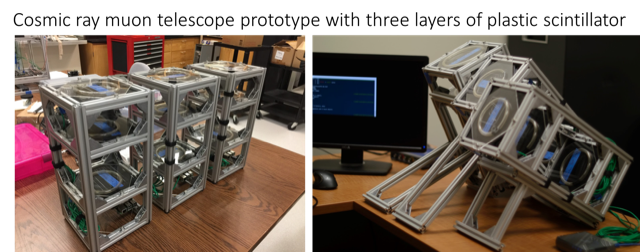
\includegraphics[width=0.95\textwidth]{images/muonTelescope1.png} 
\caption{Cosmic ray muon telescopes developed at GSU.}
\label{muonTelescope}
\end{figure}

%
%
%
\subsection{MIT Desktop Detector}
The desktop muon counter designed by developers at MIT is a self-contained, portable detector low in cost, small in scale, and minimizing in power consumption. 
%These speculations make it ideal for the expansion of cosmic ray detectors at GSU. 
The original MIT desktop detector uses a 5 x 5 x 1 cm plastic scintillator paired with a 6 x 6 mm$^2$ silicon photomultiplier (SiPM) to detect photons emitted from the absorbed energy (~1-3 MeV/cm) of minimum ionizing muon that passes through the scintillator. 
%Alpha and beta particles (other ionizing radiation particles) cannot pass through the scintillator unless they are directly on its surface. Gammas will penetrate through the detector. However, the scintillator is machined with a thickness to prevent any light produced from an occurrence from being detected. 
When a muon passes through the scintillator, the light emitted is captured by the SiPM which makes a measurable voltage pulse. This pulse is then amplified and shaped by the circuit on the main printed circuit board (PCB). Once the signal has been amplified, the amplitude of this pulse can be detected using a peak detector circuit in the main PCB so that count of photons observed by the detector, time of photon arrival, pulse amplitude, and detector dead time can be recorded by using an Arduino Nano.

 A mini-USB to USB connector and laptop can power the detector, and the data can be displayed using Linux, Mac OS Platform, or any executable program. Measurement of the total count, uptime (total runtime), and rate of counts are displayed and updated every second using an OLED screen soldered to the main PCB. Measurable occurrences can be observed visually through the LED that is soldered to the main PCB, and the LED built in the Arduino Nano. The LEDs flash every time the detector registers an event (this could be a detection of a muon or gamma), but only muon events contribute to the total count. There is a BNC connection on the main PCB, which can be used with an oscilloscope to observe raw SiPM pulses and to inject pulses to calibrate the circuit if needed when the SiPM PCB is not connected. 

%%I think most of this^can be taken out.

The desktop muon detectors built by myself and two graduate students, Ernesto Potdevin and Aisha Ahmad I Okmi, use the same components recommended by the MIT group, as well as the Desktop Muon Counter Arduino Code \cite{MIT_Code}. SensL Technologies sent the Nuclear Physics Group at GSU 3 MicroFC-60035-SMT SiPMs to use for our detectors free of charge. Using the PCB Gerber files from the MIT design, we used the manufacturer OSHPark for fabrication and depanelling of the main PCB and SiPM PCB. We use 0805 SMT components electrical components purchased from Digi-Key Electronics. I soldered each electrical component using a reflow solder at 455$^{\circ}$. The design of our detector was modified so that the main PCB is separate from the scintillator and SiPM, using electrical wires to connect the 6-pin connector on the SiPM PCB to the 6-pin header on the main PCB. This allows for open access of the Main PCB and provides future flexibility. 
\begin{figure}[htb]
\centering
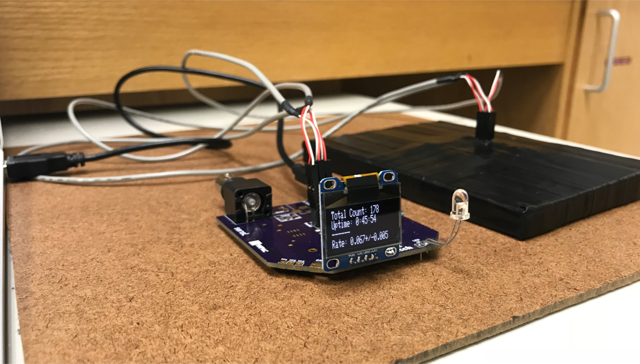
\includegraphics[width=0.75\textwidth]{images/FinalDetector_Setup.png} 
\caption{Assembled MIT version of the muon detector. The detector is being powered through the mini USB connector connected to a laptop.}
\label{MIT_WrappedScintillator}
\end{figure}


Here are a few pictures and further descriptions of the MIT detector components:
\begin{itemize}
\item {\bf Silicon photomultiplier (SiPM)} \\
The SiPM (see Figure \ref{SiPM}) produces the ADC current pulse in response to the absorption of a photon.  This SiPM provides lowest cross talk and noise. Each SiPM of this model contains 18,980 microcells of size 35\textmu, a series of avalanche photodiodes (ADP) that convert light to electricity, and four pin diodes. Only pin 1 (denoted by the white circle on the top left of silkscreen outlining SiPM shown in Figure \ref{MIT_SiPMPCB}) and pin 3 are used and soldered to the board. The anode paired with a 49.9 \textOmega \ resistor corresponds to the pin 1, and pin 3 connects the other resistors and capacitors on the SiPM circuit. 
\begin{figure}[htb]
\centering
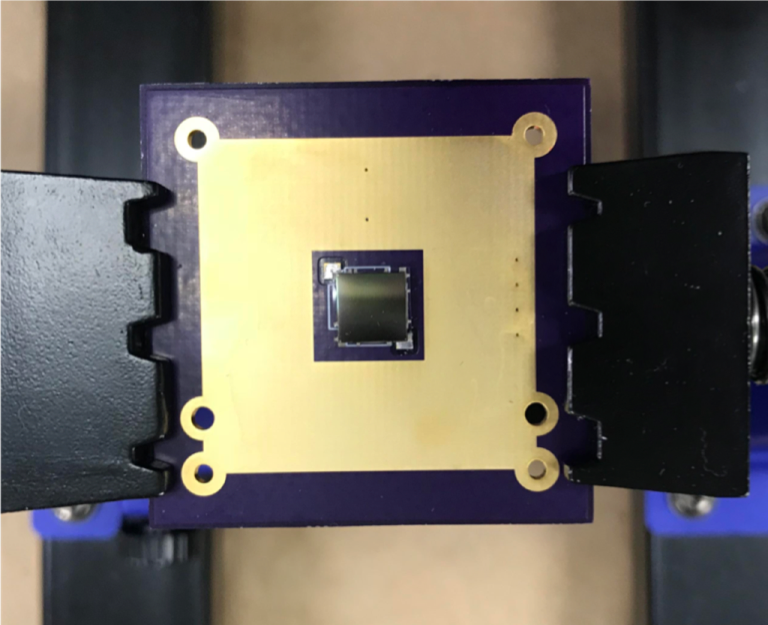
\includegraphics[width=0.60\textwidth]{images/SiPM.png} 
\caption{SensL SiPM soldered on the circuit board (center).}
\label{SiPM}
\end{figure}
\item {\bf Scintillator} \\
The dimension of the scintillator for this detector is 14 x 11 x 1 cm, as shown in Figure \ref{MIT_UScintillator}.  The Physics \& Astronomy Shop at GSU machined the scintillator, drilling four holes in a 3 x 3 cm square so that the SiPM PCB may be screwed in using 5/16" number 0 screws. After the scintillator was machined, I polished the scintillator with plastic polish and a piece of blue jean to improve its optical transparency and promote total internal reflection on the walls. This increases overall SiPM photon collection efficiency. After polishing, the scintillator is washed with dish soap and deionized water before being wrapped tight in aluminum foil,leaving an approximately 2 x 2 cm opening to mount the SiPM PCB, and then secured using black vinyl electrical tape (see Figures \ref{MIT_PScintillator} and Figure \ref{MIT_WrappedScintillator}). 
\begin{figure}[htb]
\centering
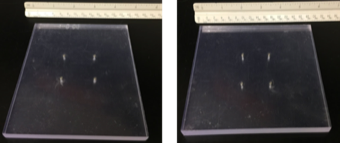
\includegraphics[width=0.95\textwidth]{images/Scintillator.png} 
\caption{Unpolished machined plastic scintillator shown to scale.}
\label{MIT_UScintillator}
\end{figure}
\begin{figure}[htb]
\centering
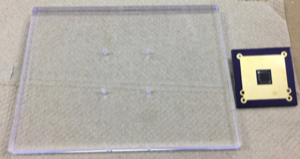
\includegraphics[width=0.95\textwidth]{images/ScintoScale.png} 
\caption{Polished plastic scintillator shown beside the populated SiPM PCB for reference.}
\label{MIT_PScintillator}
\end{figure}
\begin{figure}[htb]
\centering
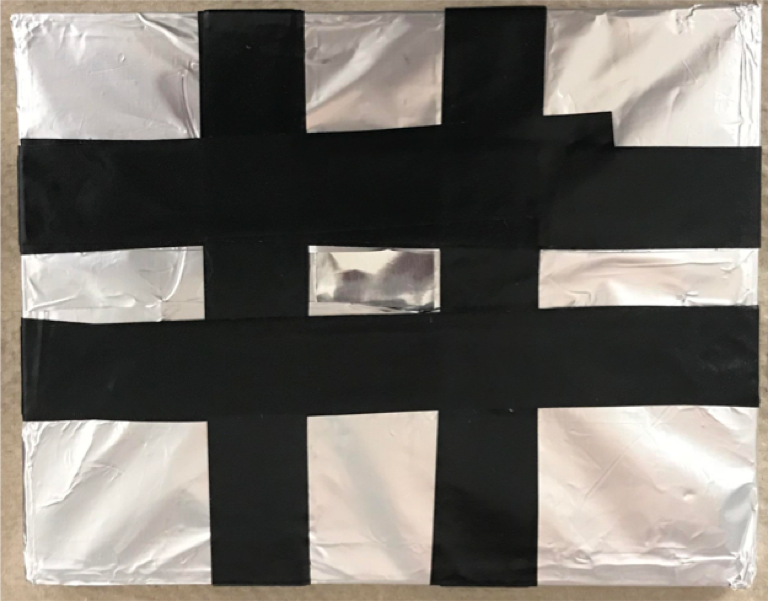
\includegraphics[width=0.75\textwidth]{images/ScintillatorWrapped.png} 
\caption{Scintillator wrapped in aluminum foil, and secured by black electrical tape with a 2cm x 2cm gap (middle) for the SiPM.}
\label{MIT_WrappedScintillator}
\end{figure}
\item {\bf SiPM PCB } \\
One muon produces around a few dozen photons. When a microcell of the SiPM absorbs light from an occurrence, it triggers a small discharge of current that will flow from pin 3 to pin 1 and continue into the circuit of the SiPM PCB. The resistors and capacitors connected to pin 3 (see Figure \ref{MIT_SiPMPCB}) are used to filter high-frequency noise in the voltage supply which might manipulate measurements. Resistor R3 (see Figure \ref{MIT_SiPMPCB_POP}) holds the line of current at the ground when no signal is detected. The six pin header shown on the top is used to connect the SiPM PCB to the main PCB. Electrical wires are used for connection to allow separation of the boards. 
Once the connection for all electrical components was made, pin 1, and 3 of the SiPM are soldered to the back of the SiPM PCB. A small amount of optical grease was applied to the surface of the SiPM before it was mounted to the scintillator. Doing so ensures that the reflective indices of both will match such that light passing through is neither reflected nor refracted. We carefully screwed the SiPM PCB into the aluminum wrapped scintillator making sure not to apply too much pressure (as it could crush the SiPM), and then wrapped the two components using black vinyl electrical tape so that no light can enter or escape. 
\begin{figure}[htb]
\centering
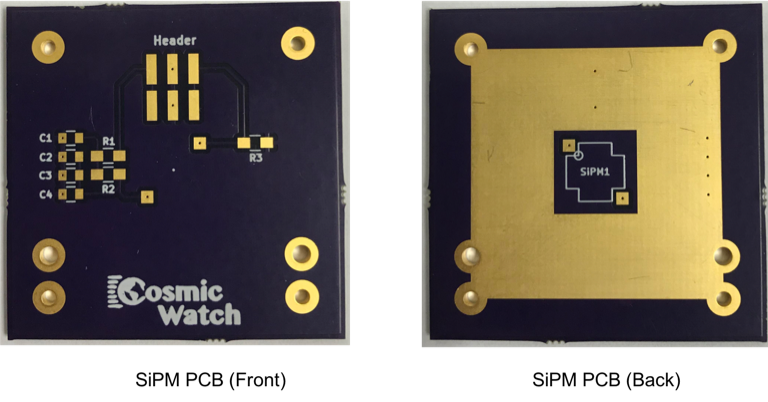
\includegraphics[width=0.75\textwidth]{images/SiPMPCB.png} 
\caption{The SiPM circuit boards without any electrical components soldered.}
\label{MIT_SiPMPCB}
\end{figure}
\begin{figure}[htb]
\centering
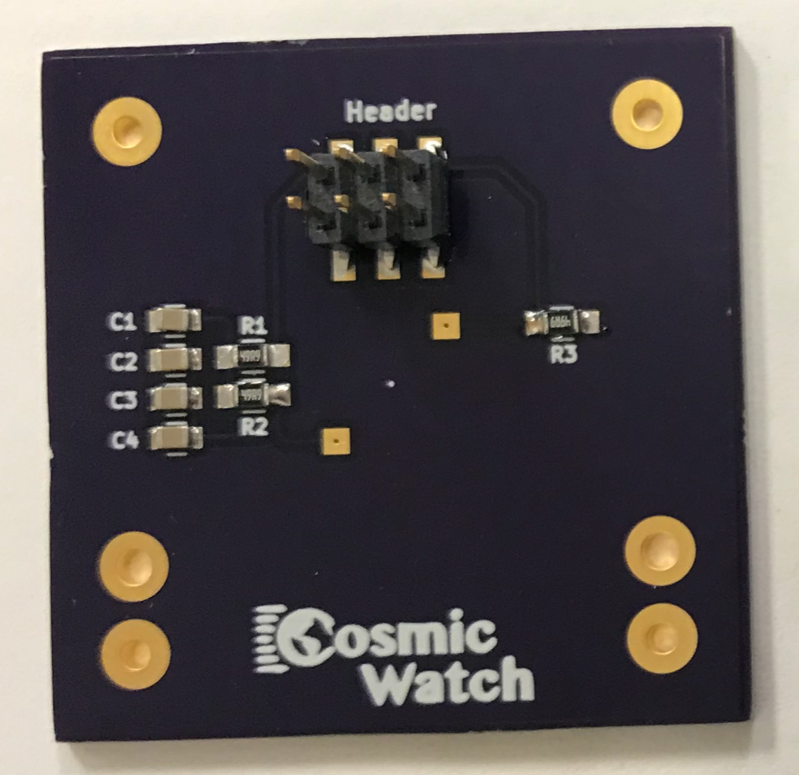
\includegraphics[width=0.65\textwidth]{images/PopSiPMPCB.png} 
\caption{The front SiPM PCB with all electrical components, including the capacitors and resistors(left) connected to pin 3 of the SiPM, the six-pin head which provides connection to the main PCB, and the 49.9 \textOmega \ resistor (right) connected to pin 1. }
\label{MIT_SiPMPCB_POP}
\end{figure}
\item {\bf Main PCB} \\
The Main PCB (see Figure \ref{MIT_mainPCB}) performs all signal processing and power regulation tasks for the detector. The bottom side of the board (see Figure \ref{MIT_mainPCB_POP}) contains the data acquisition electronics and four pin connector for the OLED screen. The top side of the board (see Figure \ref{MIT_MainSiPMPCB_POP})contains the larger components such as the OLED screen, 16 MHz Arduino Nano ATmega328, the BNC connector, and the six-pin connector. The DC-DC Booster (designed by using Linear Technology Integrated Circuit) transforms the 5 V DC, supplied by connecting the micro USB, to +29.5 V. The six-pin connector, which includes two inputs each for voltage, ground, and signal, takes this biasing voltage from the main PCB to the SiPM PCB, then also transmits the signal from the SiPM back to the main PCB. 

    Once the signal of an occurrence is transmitted back to the main PCB, it is amplified and shaped through the amplifying circuit and peak detector circuit. A factor of 20 amplifies the signal, and high-frequency amplification is omitted by a 5 pF capacitor to account for any possible error and improve voltage response. The amplified pulse is then detected and held at the level of its amplitude long enough so that the Arduino can measure its signal, then it decays and waits for the next event.

    The Arduino Nano is open-source hardware with a clock speed of 16 MHz, input voltage from around 7-12 V, and 32 KB of memory. There are two sets of the 14 digital pins (8 being analog inputs) which can be used for input and outputs, but only 7 are needed for the detector. We chose to remove the upper pins using wire cutters as they do not contribute to the detector. 

From uploading the code \cite{MIT_Code} to the  mircocontroller via micro USB, the trigger threshold on the ADC is set at approximately 23 mV, and the OLED screen and LED lights are programmed. The pulse amplitude from the peak detecting circuit is measured, and the pulse amplitude of the SiPM signal is calculated using the programmed Arduino Nano. The measured data is sent through USB connection to computer. The readout displays the total count of muon particles detected, time stamp in milliseconds, measure amplitude of ADC, calculated SiPM pulse amplitude, and dead time. The dead time is defined as the sum of time it takes the Arduino Nano to preform each operation subtracted by the total run time of the detector. 
%-------------------------------------------------------------------------- 
\begin{figure}[htb]
\centering
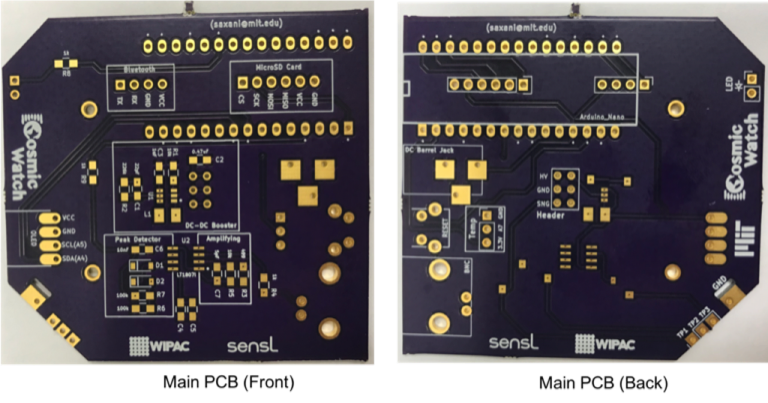
\includegraphics[width=0.98\textwidth]{images/mainPCB.png} 
\caption{Unpopulated main PCB boards with silkscreen indicating layout of components.}
\label{MIT_mainPCB}
\end{figure}
\begin{figure}[htb]
\centering
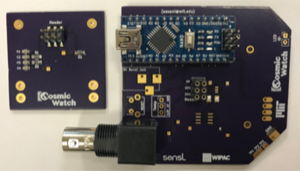
\includegraphics[width=0.75\textwidth]{images/TopMainSiPMPOP.png} 
\caption{Front of populated SiPM PCB(left) and main PCB (without LED and OLED screen components) shown side by side.}
\label{MIT_MainSiPMPCB_POP}
\end{figure}
\begin{figure}[htb]
\centering
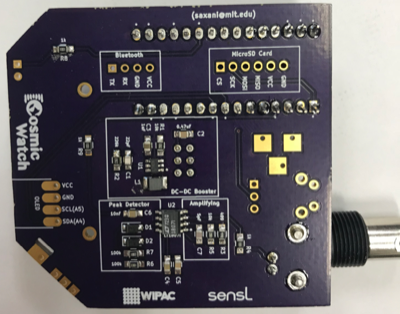
\includegraphics[width=0.65\textwidth]{images/MITMainPCBPOP.png} 
\caption{Back side of main PCB containing the majority of electrical components. Peak detector circuit (bottom left) connected to the amplifying circuit(right) by the 325 MHz OpAmp manufactured by Linear Technology.}
\label{MIT_mainPCB_POP}
\end{figure}


\end{itemize}

The desktop muon detectors built by myself and two graduate students, Ernesto Potdevin and Aisha Ahmad I Okmi, use the same components recommended by the MIT group, as well as the Desktop Muon Counter Arduino Code \cite{MIT_Code}. SensL Technologies sent the Nuclear Physics Group at GSU 3 MicroFC-60035-SMT SiPMs to use for our detectors free of charge. Using the PCB Gerber files from the MIT design, we used the manufacturer OSHPark for fabrication and depanelling of the main PCB and SiPM PCB. We use 0805 SMT components electrical components purchased from Digi-Key Electronics. I soldered each electrical component using a reflow solder at 455$^{\circ}$. The design of our detector was modified so that the main PCB is separate from the scintillator and SiPM, using electrical wires to connect the 6-pin connector on the SiPM PCB to the 6-pin header on the main PCB. This seperation allows for open access of the Main PCB and provides future flexibility. 
\begin{figure}[htb]
\centering
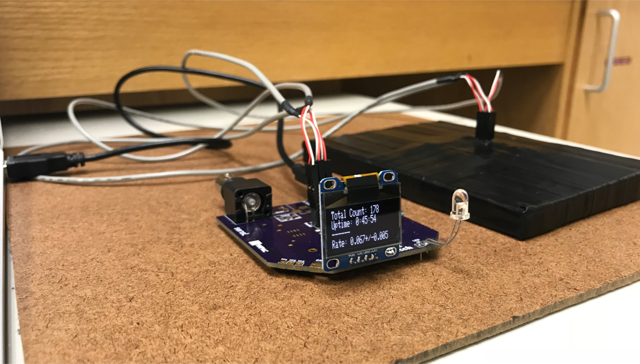
\includegraphics[width=0.75\textwidth]{images/FinalDetector_Setup.png} 
\caption{Assembled MIT version of the muon detector. The detector is being powered through the mini USB connector connected to a laptop.}
\label{MIT_WrappedScintillator}
\end{figure}


Here are a few pictures and further descriptions of the MIT detector components:
\begin{itemize}
\item {\bf Silicon photomultiplier (SiPM)} \\
The SiPM (see Figure \ref{SiPM}) produces the ADC current pulse in response to the absorption of a photon.  This SiPM provides lowest cross talk and noise. Each SiPM of this model contains 18,980 microcells of size 35\textmu, a series of avalanche photodiodes (ADP) that convert light to electricity, and four pin diodes. Only pin 1 (denoted by the white circle on the top left of silkscreen outlining SiPM shown in Figure \ref{MIT_SiPMPCB}) and pin 3 are used and soldered to the board. The anode paired with a 49.9 \textOmega \ resistor corresponds to the pin 1, and pin 3 connects the other resistors and capacitors on the SiPM circuit. 

%-------------------------------------------------------------------------- 
\begin{figure}[htb]
\centering
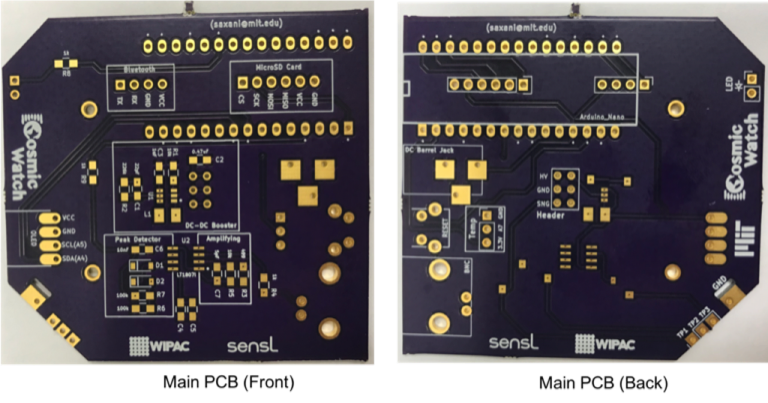
\includegraphics[width=0.98\textwidth]{images/mainPCB.png} 
\caption{Unpopulated main PCB boards with silkscreen indicating layout of components.}
\label{MIT_mainPCB}
\end{figure}
\begin{figure}[htb]
\centering
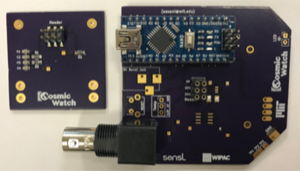
\includegraphics[width=0.75\textwidth]{images/TopMainSiPMPOP.png} 
\caption{Front of populated SiPM PCB(left) and main PCB (without LED and OLED screen components) shown side by side.}
\label{MIT_MainSiPMPCB_POP}
\end{figure}
\begin{figure}[htb]
\centering
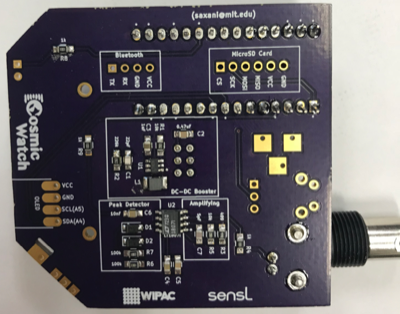
\includegraphics[width=0.65\textwidth]{images/MITMainPCBPOP.png} 
\caption{Back side of main PCB containing the majority of electrical components. Peak detector circuit (bottom left) connected to the amplifying circuit(right) by the 325 MHz OpAmp manufactured by Linear Technology.}
\label{MIT_mainPCB_POP}
\end{figure}


\end{itemize}

\section{Test of MIT Detector}
After populating the boards with all of the electronic components, each connection was checked using a multi-meter. The DC-DC Booster connection on the main PCB was tested without the SiPM PCB (See Figure \ref{Bias Voltage check}) and found to have to correct biasing voltage required, confirming that all the components of the main PCB are correctly soldered, and the detector is ready for assembly.

    From plugging in the constructed detector, the OLED screen appears, signifying it is running.  Every 5.8 \textmu s measurements are recorded, which is longer than the length of the peak detector pulse; therefore, the initial few measurements appear constantly and are excluded when analyzing muon counts. The trigger pulse time has an uncertainty of 0.4 \textmu s, and using the laptop for readout adds an additional uncertainty of 0.1 ms. 

    Measurements were conducted in the basement of the Natural Science Center at GSU, and the rate of muon counts per second was found to be 0.5 +/- 0.007. When the detector was taken outside for measurements, the rate of muon counts increased by a factor of 2. These results are consistent with what we expected; however, the dead time for both ranged from 1,000-55,000 ms. An appropriate dead time would be less than 1,000 ms. Therefore, further modifications will be needed to decrease the time it takes the Arduino to perform tasks prompted by the code before testing the detector's efficiency against the cosmic ray muon telescope. 

    To accurately obtain significant data to test the detector's performance, we will need to eliminate the effects of atmospheric pressure and record data for seven days or more. The current code does not include a function to save the output to a text file,  deleting measurements displayed through a terminal window as time progresses. This poses a difficulty on consistently recording data for the appropriate length of time.  Therefore, additional modifications on the detector are needed as well. 
\begin{figure}[htb]
\centering
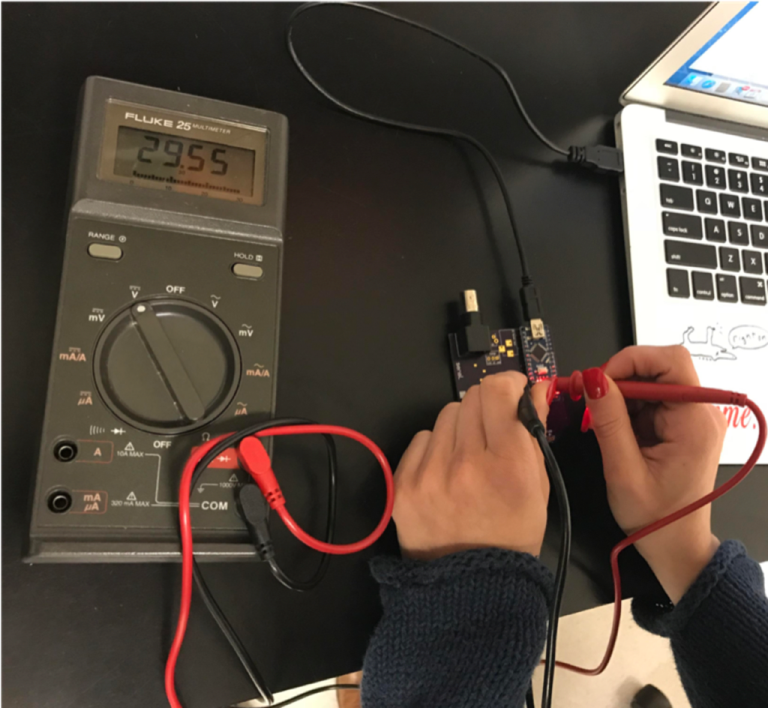
\includegraphics[width=0.75\textwidth]{images/VoltageReading.png} 
\caption{Biasing voltage being check by connecting a multi-meter between the HV pin and ground of the 6-pin header on main PCB.}
\label{Bias Voltage check}
\end{figure}
\begin{figure}[htb]
\centering
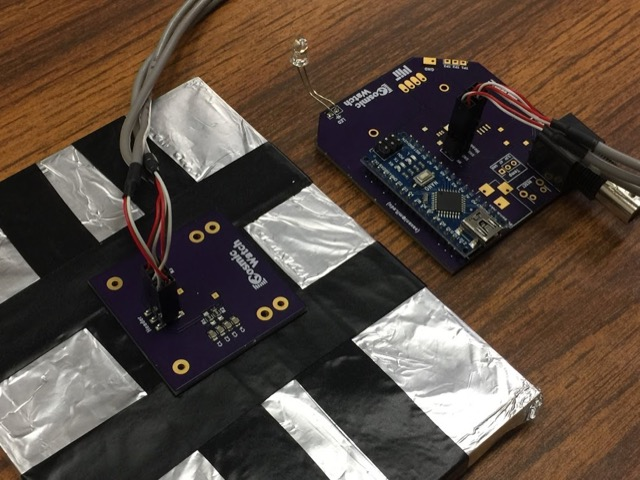
\includegraphics[width=0.75\textwidth]{images/Connection_PCB.jpg} 
\caption{Connection of the six-pin header on the SiPM PCB to the six-pin connector on the main PCB using electrical wires is shown prior to wrapping the scintillator and SiPM PCB light tight with electrical tape.}
\end{figure}
\section{Summary}
The MIT cosmic ray muon detector provided measurements efficiently and simply. The simple design makes for a quick build at a low price; we were able to build our detector for under \$70 each. However, the Arduino Nano does impose some restrictions. There is an uncertainty of +/- 50 ppm with the time of measurements, such that the first three muon counts are not accurate. The current code does not provide room for expansion of functionalities, as it currently occupies 60\% of memory space and 49\% of the dynamic memory while requiring that storage space and remaining dynamic memory be less that 70\%.  Components, such as the OLED screen and LED lights, are contributing to the significantly high dead time. To maintain their use while minimizing the dead time, we will need to add additional hardware to expand the capabilities of the detector. Connecting the Arduino Nano to another microcontroller, the Raspberry Pi, and modifying its code will eliminate these issues. Also, the Raspberry Pi has many built-in functionalities that could further enhance the detector to provide more meaningful measurements. The Raspberry Pi can work as the power supply for the detector, which will allow us to record data without having to monitor the readout on our laptop. Instead, data can be stored to an SD card on the Raspberry Pi and viewed later. These modifications will allow us to record muon occurrence for more than seven days. Through further analysis using an oscilloscope, I determined that the MIT design of directly coupling the SiPM to the scintillator provided data inconsistencies when oriented vertically. This finding gave myself, and my advisor Dr. He, the certainty that the GSU Muon Telescope is the best-suited detector for correlation study of cosmic ray flux and atmospheric and space weather. 
\clearpage
\newpage
%%%%%%%%%%%%%%%%%%%%%%%
\bibliographystyle{unsrt}%
\bibliography{main} % The file containing the bibliography

\end{document}
